\chapter{Proposed Architectural Design}

\section{System Overview}
The proposed condition-wise healthcare system with blockchain integration aims to deliver high-assurance data management without sacrificing system resilience. The core design philosophy centers on achieving ``defense in depth'' by physically and logically segregating the Trusted Authority (TA) services from the Hyperledger Fabric blockchain ordering consensus nodes. The overall data flow involves several meticulously designed components encompassing external interfaces, an LLM-based priority engine, cryptographic secret custodians, and an off-chain secure object store.

\section{Component Architecture}
The architecture defines interactions between several high-level actors and services \cite{kumar2022fog}.

\subsection{Hospital Node / Uploader}
Hospitals serve as the localized points of patient data ingestion. Medical staff upload unstructured EHR reports directly into the application endpoint. The frontend ensures secure session handling via standard web-security protocols \cite{torongo2023decentralized}.

\subsection{Trusted Authority (TA) Service}
The TA operates as an independent backend orchestration service. Unlike theoretical ``Orderer-as-TA'' models where cryptographic responsibilities are dangerously colocated with the blockchain's core consensus, our design extracts the TA into a separate runtime boundary. The TA is fundamentally responsible for:
\begin{itemize}
    \item Interfacing with the LLM API for priority classification.
    \item Generating unique, condition-specific symmetric keys utilizing pseudorandom numbers.
    \item Applying AES-GCM authenticated encryption algorithms across incoming EHR texts.
    \item Slicing the symmetric key using Shamir's threshold algorithms.
    \item Orchestrating the retrieval and reconstruction phases over secure REST pathways.
\end{itemize}

\subsection{Hyperledger Fabric Network}
A localized Hyperledger Fabric network acts as the system's ledger. It contains peer organizations (e.g., \texttt{Org1MSP}) running smart contracts (chaincode). The ledger essentially stores JSON-formatted metadata structures describing the versioning of the document, the cryptographic threshold indices, and securely wrapped shares. Importantly, raw data and raw encryption keys never touch the ledger, ensuring data privacy standards are strictly upheld.

\subsection{Off-Chain Object Store}
Encrypted ciphertext and nonce parameters are directed towards an auxiliary off-chain storage pool (an Object Store). Segregating the high-volume payload from the ledger optimizes the blockchain's performance by minimizing state bloating.

\section{Condition-Wise Granularity}
One of the most consequential design decisions is the implementation of condition-wise access control. Patient datasets are conceptually split by condition namespaces (e.g., \texttt{P001\_cardiology}, \texttt{P001\_oncology}). Distinct conditions are encrypted with completely uncorrelated AES-GCM keys. Therefore, providing a doctor with the capability to reconstruct the cardiology key structurally provides absolutely zero mathematical leverage toward discovering the oncology key.

\section{Data Flow Description}

The upload routine proceeds sequentially:
\begin{enumerate}
    \item \textbf{Data Ingestion:} The Hospital uploads medical records into the TA module.
    \item \textbf{Priority Assessment:} The TA parses the data through an LLM layer, returning an urgency score (\texttt{LOW}, \texttt{MEDIUM}, or \texttt{HIGH}).
    \item \textbf{Threshold Determination:} Based on priority, the TA evaluates the integer $k$, representing the minimum number of nodes needed for reconstruction.
    \item \textbf{Encryption Operation:} An AES-GCM sub-key is generated. The ciphertext is deployed into the off-chain store.
    \item \textbf{Key Distribution:} The AES-GCM key is fed into Shamir's Secret Sharing to yield $n$ shares.
    \item \textbf{NMK Wrapping:} Each share is independently encrypted (wrapped) with the specific Node Master Key (NMK) corresponding to each peer in the cluster.
    \item \textbf{Auditing to Blockchain:} Metadata encapsulating the condition mappings, threshold logic, and the NMK-wrapped shares are relayed through the Fabric Gateway to be immortalized on the ledger \cite{rahman2019secure}.
\end{enumerate}

In Phase 2.2, the evaluation workflow was extended with a dataset-style input option to better reflect realistic usage. A patient document simulation module generates structured patient documents (patient name, disease label, and priority), and a persistent disease-to-numeric identifier mapping is used to standardize record identifiers. For simulated uploads, record keys are generated in the format \texttt{<patient\_number>\_<disease\_id>} (e.g., \texttt{21\_5}), which preserves compatibility with existing parsing and storage logic.

\begin{figure}[ht]
\begin{center}
  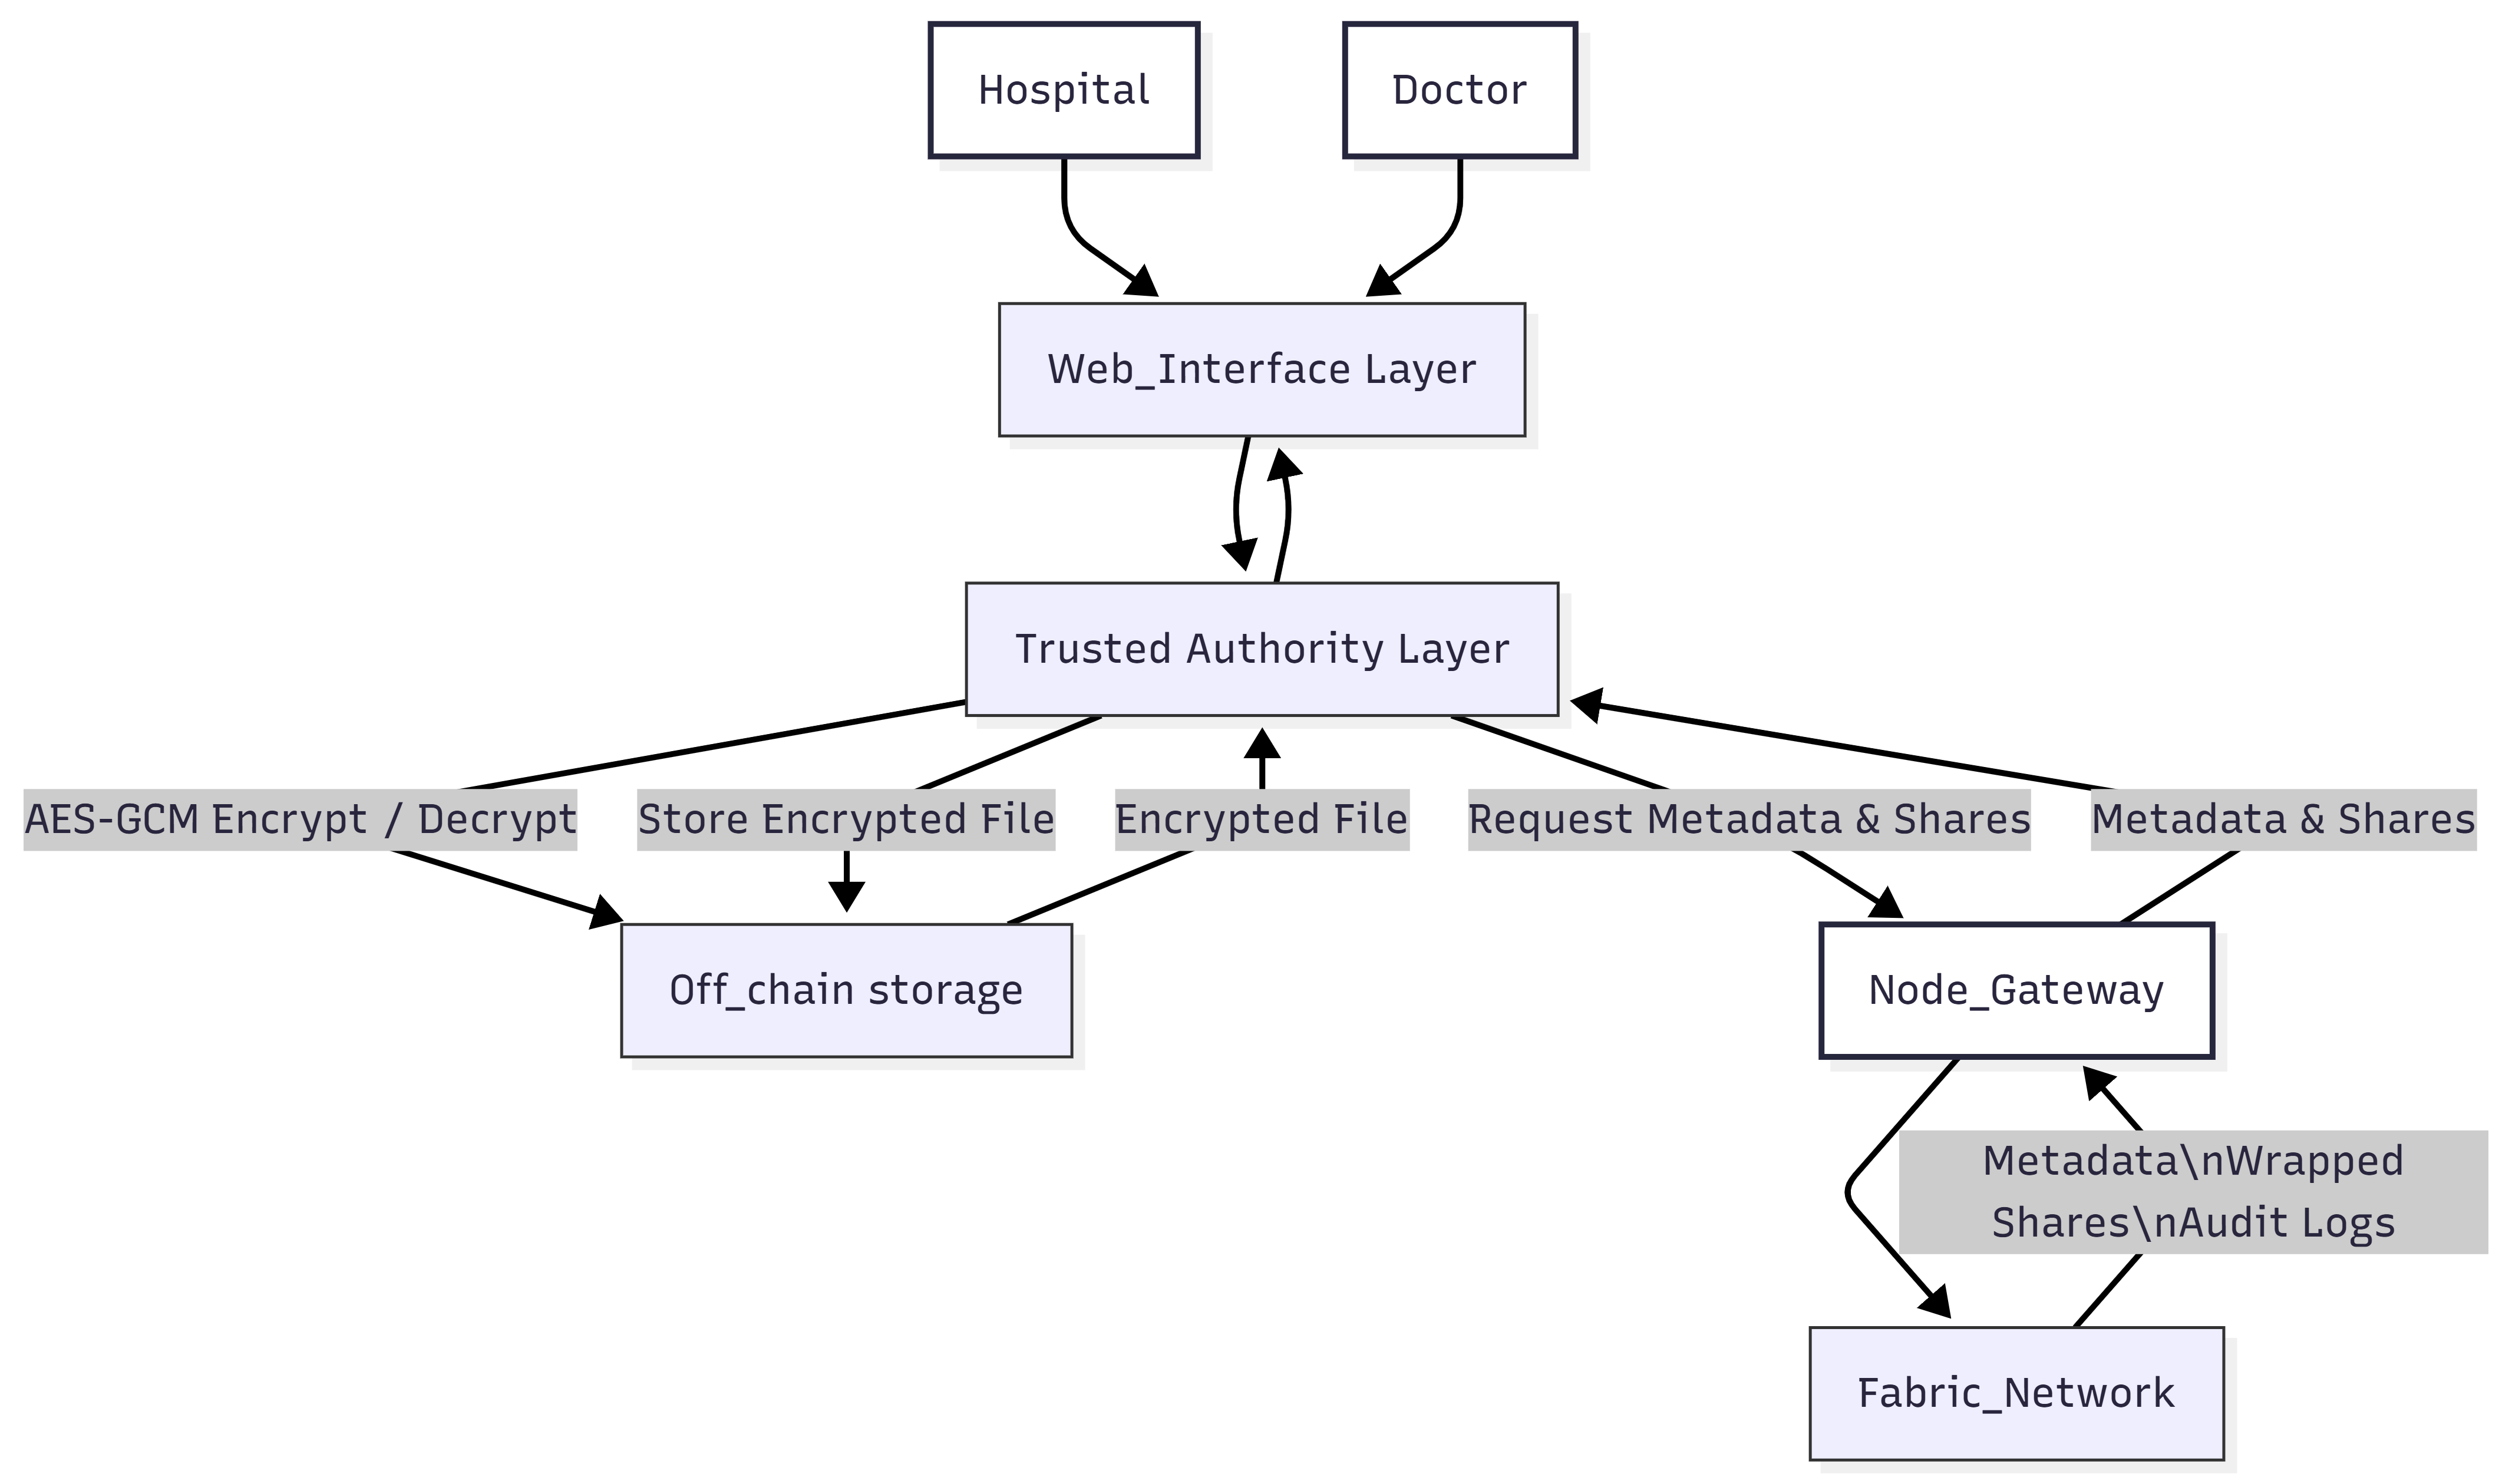
\includegraphics[width=12cm]{system_flow_phase2_1.png}
\end{center}
\caption{Overall System Data Flow showing off-chain storage and Fabric metadata}
\label{Fig:SystemFlow}
\end{figure}

The retrieval process essentially runs in reverse. An authenticated doctor issues a view request. The TA queries the Fabric ledger for metadata, retrieves the $k$ required wrapped shares, contacts the peer nodes to temporarily unwrap those pieces, reconstructs the AES sub-key, fetches the ciphertext from the object store, decrypts the contents, and furnishes the plaintext report.

\begin{figure}[ht]
\begin{center}
  \includegraphics[width=12cm]{LLD_flow_phase2_1.png}
\end{center}
\caption{Detailed Low Level Architecture Diagram for Blockchain Operations}
\label{Fig:LLDFlow}
\end{figure}

\section{Security Architecture Implications}
This architecture meticulously avoids standard centralized fallacies. Even if an adversary compromises a Fabric peer node, they only attain NMK-wrapped shares belonging to other nodes. Since the $n$ shares are individually sealed by distinct node credentials, a single node's compromise prevents the adversary from piecing together the required $k$ shares. This effectively converts the blockchain into a distributed, cooperative cryptographic lockbox.
